%% (2) Build options: PdfLaTex + BibTex

\documentclass[]{article}
\usepackage[T1]{fontenc}
\usepackage[round]{natbib}
\bibliographystyle{plainnat}

\usepackage[pass]{geometry}
\usepackage[table]{xcolor} %
\usepackage{booktabs}	% Tables
\usepackage{arydshln} 	% dashed lines in tables
\usepackage{pdflscape}	% Landscape page

\usepackage{caption}
\usepackage{subcaption}
\usepackage{amsfonts}
\usepackage{setspace}
\usepackage[spaces, hyphens]{url}
\usepackage[colorlinks, allcolors=blue]{hyperref} 

% Macros
\newcolumntype{L}[1]{>{\raggedright\let\newline\\\arraybackslash\hspace{0pt}}m{#1}}
\newcolumntype{C}[1]{>{\centering\let\newline\\\arraybackslash\hspace{0pt}}m{#1}}
\newcolumntype{R}[1]{>{\raggedleft\let\newline\\\arraybackslash\hspace{0pt}}m{#1}}
\newcommand{\rowspace}[1]{\renewcommand{\arraystretch}{#1}}

%opening
\title{An empirical study of the na\"ive REINFORCE algorithm for predictive maintenance of industrial machines}
\author{Rajesh Siraskar}

\onehalfspacing

\begin{document}

\maketitle

\begin{abstract}
The 14th-century friar, William of Ockham, has been attributed for giving us the "Occam's razor" principle -- when there are two competing "theories" predicting the same phenomenon, one should prefer the \textit{simpler} of two.

In this empirical study, we document the performance of a simple, early reinforcement learning algorithm, REINFORCE, implemented for a predictive maintenance problem. We compare a very naive implementation of REINFORCE against the predictions of industry-grade Stable-Baselines3 (SB-3) implementations of three advanced algorithms, namely, Deep Q-Network (DQN), Advantage Actor-Critic (A2C) and Proximal Policy Optimization (PPO). Our broad goal was to understand the performance under various scenarios such as a simulation-based environment, three sets of real tool-wear data, added noise levels, and a random chance of break-down. Model performance was measured by how accurately the predictive maintenance agent suggested tool replacement compared to a deterministic preventive maintenance rule based on the tool-wear threshold. 

Our findings indicate that the REINFORCE performs significantly well for this particular problem. Across variants of the environment, the REINFORCE algorithm demonstrated an average F1 performance of 0.836 against 0.383 for A2C, 0.471 for DQN, and 0.402 for PPO. As a measure of stability, the overall standard deviation for REINFORCE was 0.041, while A2C, DQN, and PPO standard deviations were 0.059, 0.029, and 0.070, respectively. Across precision on tool replacement, REINFORCE was better by 0.354 basis points than the best of advanced algorithms and demonstrated a variance lower by 0.004. While the REINFORCE demonstrated better performance for each variant, it was observed that the training was unstable, occasionally producing poor performance models. On the other hand, the SB-3 implementations training was more stable, almost always producing models with an F1 in the range 0.47-0.50.


\end{abstract}


\section{Method and Inference}
\begin{itemize}
	\item why classifction metrics
	\item why F1beta
\end{itemize}

\subsection{Method - training and testing}

\begin{itemize}
	\item Training: SB-3 - 10 k eps. 3 times. Average their outputs
	\item Testing: 
	\begin{itemize}
		\item Avg. over 5 rounds.
		\item Each round - avg over 40 test cases x 10 test rounds
		\item Total: 40 x 10 x 5 = 2000 cases
		\item Avgs over: 10 rounds (of 40 cases each) X 5 rounds of \textbf{re-trained} SB-3 agents = 50 rounds 
	\end{itemize}
\end{itemize}

\subsection{Inference}
\begin{itemize}
	\item Training: SB-3 is also unstable - show examples of results such as A2C/DQN 0.00 
	\item Training: SB-3 is also unstable - SHOW SB-3 tensorboard plots
	\item Training: SB-3 is also unstable - EXCEL plots of results over the 10 rounds 	
\end{itemize}


\section{Introduction}
Introduced in 1992, the REINFORCE algorithm is considered as a basic reinforcement learning algorithm. It is a policy-based, on-policy as well as off-policy algorithm, capable of handling both discrete and continuous observation and action domains.

In practice the REINFORCE algorithm is considered as ``weak" learner and superseded by several algorithms developed since. Most notably the Q-Learning and its deep-neural network version, the DQN, followed by Actor-Critic and one of the most robust modern day algorithms, the PPO. 

\href{https://www.ri.cmu.edu/pub_files/2013/7/Kober_IJRR_2013.pdf}{Reinforcement Learning in Robotics: A Survey}  - Jens Kober J. Andrew Bagnell Jan Peters -   
Initial gradient-based approaches such as finite differences gradients or REINFORCE
(Williams, 1992) have been rather slow. The weight perturbation algorithm is related to
REINFORCE but can deal with non-Gaussian distributions which significantly improves
the signal to noise ratio of the gradient (Roberts et al., 2010). Recent natural policy
gradient approaches (Peters and Schaal, 2008c,b) have allowed for faster convergence
which may be advantageous for robotics as it reduces the learning time and required
real-world interactions.

	
\section{Hyper-parmeters}

\begin{table*}\centering
	\sffamily
	\rowspace{1.5}
	\begin{tabular}{L{2cm} R{2.5cm} R{2.5cm} R{2.5cm} R{3cm}}
		\arrayrulecolor{black!40}\toprule
		&\textbf{A2C}&\textbf{DQN}&\textbf{PPO}&\textbf{REINFORCE}\\ \midrule
		
		Network\par architecture&input dim x\par [64|Tanh x 64|Tanh]\par x output dim&input dim x\par [64|Tanh x 64|Tanh]\par x output dim&input dim x\par [64|Tanh x 64|Tanh]\par x output dim&input dim x\par [64|ReLU]\par x output dim\\
		Layers&2&2&2&1\\
		Units&64  x 64&64  x 64&64  x 64&64\\
		Activation&Tanh, Tanh&Tanh, Tanh&Tanh, Tanh&ReLU\\
		Learning rate&0.0007&0.0001&0.0003&0.01\\
		Gamma&0.99&0.99&0.99&0.99\\
		Optimizer&RMSprop&Adam&Adam&Adam\\
			
		\bottomrule
	\end{tabular}
	\caption{Hyper-parameters of the RL algorithms}
	\label{tbl:hyperparameters}
\end{table*}



soure of ppo implementation details \url{https://iclr-blog-track.github.io/2022/03/25/ppo-implementation-details/}

source of SB-3 network mp : \url{https://github.com/openai/baselines/blob/ea25b9e8b234e6ee1bca43083f8f3cf974143998/baselines/common/models.py#L75-L103}

\subsection{PPO hyperparms}

implementation guide source >> https://iclr-blog-track.github.io/2022/03/25/ppo-implementation-details/

By default, PPO uses a simple MLP network consisting of two layers of 64 neurons and Hyperbolic Tangent as the activation function. Then PPO builds a policy head and value head that share the outputs of the MLP network. Below is a pseudocode:
%\textt{
%network = Sequential(
%layer_init(Linear(np.array(envs.single_observation_space.shape).prod(), 64)),
%Tanh(),
%layer_init(Linear(64, 64)),
%Tanh(),
%)
%value_head = layer_init(Linear(64, 1), std=1.0)
%policy_head = layer_init(Linear(64, envs.single_action_space.n), std=0.01)
%hidden = network(observation)
%value = value_head(hidden)
%action = Categorical(policy_head(hidden)).sample()}

\subsection{dqn hyperparms}


default hyperparms : \url{https://stable-baselines3.readthedocs.io/en/master/_modules/stable_baselines3/common/policies.html}

overridden in indiv policies for example 
SB3 DQN hypoerparms for example were taken from ;
Paper: https://arxiv.org/abs/1312.5602, https://www.nature.com/articles/nature14236
Default hyperparameters are taken from the Nature paper,
except for the optimizer and learning rate that were taken from Stable Baselines defaults



\section{Results}
\subsection{Detailed metrics}
\newgeometry{margin=2cm} % Change margins for landscape table
\begin{landscape}\centering
	\begin{table*}
		\sffamily
		\rowspace{1.3}
		\begin{tabular}{@{}l rrrr c rrrr c rrrr c rrrr@{}} \arrayrulecolor{black!40}\toprule
			& \multicolumn{4}{c}{\textbf{REINFORCE}} & & \multicolumn{4}{c}{A2C} &
			& \multicolumn{4}{c}{DQN} & & \multicolumn{4}{c}{PPO} \\
			\cmidrule{2-5} \cmidrule{7-10} \cmidrule{12-15} \cmidrule{17-20}
			Environment &Prec. &Recall &F1 &F0.5 & &Prec. &Recall &F1 &F0.5 & &Prec. &Recall &F1 &F0.5 & &Prec. &Recall &F1 &F0.5\\ \midrule
			
			Simulated  - No noise &0.999 &0.645 &0.782 & 0.898 & & 0.335 &0.359 &0.344 &0.338 & &0.348 &0.597 &0.410 &0.352 & &0.392 &0.211 &0.252&0.303\\
			Simulated  - Low noise &0.943 &0.954 &0.948 & 0.945 & & 0.409 &0.318 &0.349 &0.379 & &0.273 &0.064 &0.076 &0.108 & &0.359 &0.173 &0.205&0.255\\
			Simulated  - High noise &0.889 &0.974 &0.929 & 0.904 & & 0.471 &0.439 &0.443 &0.455 & &0.423 &0.408 &0.295 &0.284 & &0.402 &0.205 &0.248&0.307\\ \midrule
			
			PHM C01 SS - No noise &0.886 &0.978 &0.928 & 0.902 & & 0.294 &0.337 &0.305 &0.296 & &0.350 &0.405 &0.291 &0.269 & &0.517 &0.494 &0.471&0.476\\
			PHM C01 SS - Low noise &0.916 &0.893 &0.903 & 0.911 & & 0.526 &0.645 &0.568 &0.540 & &0.321 &0.591 &0.404 &0.343 & &0.490 &0.415 &0.443&0.468\\
			PHM C01 SS - High noise &0.757 &0.926 &0.831 & 0.784 & & 0.499 &0.632 &0.542 &0.513 & &0.399 &0.402 &0.308 &0.292 & &0.403 &0.223 &0.270&0.325\\ \hdashline
			
			PHM C04 SS - No noise &0.865 &0.959 &0.908 & 0.881 & & 0.515 &0.676 &0.575 &0.535 & &0.365 &0.497 &0.383 &0.348 & &0.431 &0.239 &0.265&0.311\\
			PHM C04 SS - Low noise &0.722 &0.980 &0.831 & 0.762 & & 0.399 &0.393 &0.391 &0.393 & &0.409 &0.589 &0.410 &0.361 & &0.438 &0.299 &0.334&0.377\\
			PHM C04 SS - High noise &0.770 &0.809 &0.787 & 0.776 & & 0.375 &0.456 &0.397 &0.381 & &0.408 &0.411 &0.296 &0.282 & &0.491 &0.324 &0.362&0.409\\ \hdashline
			
			PHM C06 SS - No noise &0.996 &0.609 &0.751 & 0.879 & & 0.463 &0.454 &0.455 &0.459 & &0.538 &0.780 &0.585 &0.523 & &0.402 &0.410 &0.374&0.370\\
			PHM C06 SS - Low noise &0.968 &0.854 &0.905 & 0.941 & & 0.508 &0.615 &0.548 &0.522 & &0.395 &0.593 &0.411 &0.362 & &0.454 &0.342 &0.367&0.404\\
			PHM C06 SS - High noise &0.699 &0.912 &0.790 & 0.732 & & 0.480 &0.512 &0.466 &0.467 & &0.581 &0.499 &0.417 &0.433 & &0.424 &0.199 &0.252&0.314\\ \midrule
			
			PHM C01 MS - No noise &0.824 &0.895 &0.856 & 0.836 & & 0.444 &0.284 &0.315 &0.358 & &0.313 &0.215 &0.165 &0.175 & &0.513 &0.347 &0.395&0.448\\
			PHM C04 MS - No noise &0.752 &0.678 &0.709 & 0.733 & & 0.506 &0.326 &0.368 &0.425 & &0.588 &0.642 &0.492 &0.486 & &0.472 &0.455 &0.444&0.452\\
			PHM C06 MS - No noise &1.000 &0.643 &0.779 & 0.896 & & 0.499 &0.731 &0.575 &0.523 & &0.520 &0.239 &0.209 &0.256 & &0.509 &0.260 &0.330&0.409\\
					
			\bottomrule
		\end{tabular}
		\caption{Model performance comparison all variants of the environments.}
		\label{tbl:DetailedMetrics}
	\end{table*}
\end{landscape}
\restoregeometry % Restore margins after landscape table

\subsection{Overall summary performance}
\begin{table*}[hbt!]\centering
	\sffamily
	\rowspace{1.3}
	\begin{tabular}{@{}l rr c rr c rr c rr@{}}
		\arrayrulecolor{black!40}\toprule
		& \multicolumn{2}{c}{Precision} & \phantom{i} & \multicolumn{2}{c}{Recall} & \phantom{i} & \multicolumn{2}{c}{F1-score} & \phantom{i} & \multicolumn{2}{c}{F1-beta score} \\
		\cmidrule{2-3} \cmidrule{5-6} \cmidrule{8-9} \cmidrule{11-12} 
		
		&Mean &SD & &Mean &SD & &Mean &SD& &Mean & SD\\ \midrule
		A2C & 0.448 & 0.074 & &0.478 & 0.084 & & 0.443 & 0.071 & &0.439 &0.069 \\
		DQN & 0.415 & 0.196 & &0.462 & 0.033 & & 0.343 & 0.038 & &0.325 &0.063 \\
		PPO & 0.447 & 0.147 & &0.306 & 0.090 & & 0.334 & 0.093 & &0.375 &0.107 \\
		REINFORCE & 0.866 & 0.042 & &0.847 & 0.054 & & 0.842 & 0.043 & &0.852 &0.042 \\	
		\bottomrule
	\end{tabular}
	\caption{Model performance summary - averaged over all environment.}
	\label{tbl:OverallSummary}
\end{table*}

\subsection{Simulated environment}
\begin{table*}[hbt!]\centering\sffamily
	\rowspace{1.3}
	\begin{tabular}{@{}l rr c rr c rr c rr@{}}
		\arrayrulecolor{black!40}\toprule
		& \multicolumn{2}{c}{Precision} & \phantom{i} & \multicolumn{2}{c}{Recall} & \phantom{i} & \multicolumn{2}{c}{F1-score} & \phantom{i} & \multicolumn{2}{c}{F1-beta score} \\
		\cmidrule{2-3} \cmidrule{5-6} \cmidrule{8-9} \cmidrule{11-12} 
		
		&Mean &SD & &Mean &SD & &Mean &SD& &Mean & SD\\ \midrule
		A2C & 0.405 & 0.079 & &0.372 & 0.086 & & 0.379 & 0.076 & &0.391 &0.076 \\
		DQN & 0.348 & 0.217 & &0.356 & 0.033 & & 0.260 & 0.041 & &0.248 &0.068 \\
		PPO & 0.385 & 0.175 & &0.196 & 0.064 & & 0.235 & 0.080 & &0.289 &0.110 \\
		REINFORCE & 0.944 & 0.029 & &0.858 & 0.041 & & 0.886 & 0.032 & &0.916 &0.030 \\
		\bottomrule
	\end{tabular}
	\caption{Model performance summary - averaged over simulated environments.}
	\label{tbl:SimulatedEnv}
\end{table*}

\newpage
\subsection{Real data -- simple single-variable environment}
\begin{table*}[h]\centering
	\sffamily
	\rowspace{1.3}
	\begin{tabular}{@{}l rr c rr c rr c rr@{}}
		\arrayrulecolor{black!40}\toprule
		& \multicolumn{2}{c}{Precision} & \phantom{i} & \multicolumn{2}{c}{Recall} & \phantom{i} & \multicolumn{2}{c}{F1-score} & \phantom{i} & \multicolumn{2}{c}{F1-beta score} \\
		\cmidrule{2-3} \cmidrule{5-6} \cmidrule{8-9} \cmidrule{11-12} 
		
		&Mean &SD & &Mean &SD & &Mean &SD& &Mean & SD\\ \midrule
		A2C & 0.451 & 0.064 & &0.524 & 0.085 & & 0.472 & 0.067 & &0.456 &0.063 \\
		DQN & 0.418 & 0.172 & &0.530 & 0.032 & & 0.389 & 0.034 & &0.357 &0.055 \\
		PPO & 0.450 & 0.146 & &0.327 & 0.095 & & 0.349 & 0.095 & &0.384 &0.106 \\
		REINFORCE & 0.842 & 0.043 & &0.880 & 0.053 & & 0.848 & 0.043 & &0.841 &0.042 \\
		\bottomrule
	\end{tabular}
	\caption{Model performance summary - averaged over PHM-2010 environments with simple single-variable environment.}
	\label{tbl:PHMSS}
\end{table*}

\subsection{Real data -- complex multi-variate environment}
\begin{table*}[hbt!]\centering
	\sffamily
	\rowspace{1.3}
	\begin{tabular}{@{}l rr c rr c rr c rr@{}}
		\arrayrulecolor{black!40}\toprule
		& \multicolumn{2}{c}{Precision} & \phantom{i} & \multicolumn{2}{c}{Recall} & \phantom{i} & \multicolumn{2}{c}{F1-score} & \phantom{i} & \multicolumn{2}{c}{F1-beta score} \\
		\cmidrule{2-3} \cmidrule{5-6} \cmidrule{8-9} \cmidrule{11-12} 
		
		&Mean &SD & &Mean &SD & &Mean &SD& &Mean & SD\\ \midrule
		A2C & 0.483 & 0.101 & &0.447 & 0.081 & & 0.419 & 0.075 & &0.435 &0.079 \\
		DQN & 0.474 & 0.248 & &0.365 & 0.038 & & 0.289 & 0.049 & &0.306 &0.082 \\
		PPO & 0.498 & 0.121 & &0.354 & 0.103 & & 0.390 & 0.101 & &0.436 &0.104 \\
		REINFORCE & 0.859 & 0.053 & &0.739 & 0.069 & & 0.781 & 0.055 & &0.822 &0.052 \\
		\bottomrule
	\end{tabular}
	\caption{Model performance summary - averaged over PHM-2010 environments with complex multi-variate environment.}
	\label{tbl:PHMMS}
\end{table*}


\section{Stable Baseline algorithms - default architectures}

\section{A2C - architecture}
\textbf{Actor-Critic Policy}: Two fully interconnected layers of 64 units with tanh activation.
\begin{itemize}
	\item Policy network:
	\begin{itemize}
		\item Linear (input dimensions = 2, output dimensions = 64, bias=True)
		\item Tanh()
		\item Linear(input dimensions = 64, output dimensions = 64, bias=True)
		\item Tanh()
	\end{itemize}

	\item Value network:
	\begin{itemize}
		\item Linear(input dimensions = 2, output dimensions = 64, bias=True)
		\item Tanh()
		\item Linear(input dimensions = 64, output dimensions = 64, bias=True)
		\item Tanh()
	\end{itemize}
\end{itemize}


%\begin{table*}[hbt!]\centering
%	\rowspace{1.3}
%	\begin{tabular}{@{}l rr c rr c rr@{}}
%		\arrayrulecolor{black!40}\toprule
%		& \multicolumn{2}{c}{Precision} & \phantom{i} & \multicolumn{2}{c}{Recall} & \phantom{i} & \multicolumn{2}{c}{F1-score} \\
%		\cmidrule{2-3} \cmidrule{5-6} \cmidrule{8-9} 
%		%Model &Precision &Recall &F1 &  &Precision &Recall &F1 & &Precision &Recall &F1 & &Precision &Recall &F1\\ \midrule
%		
%		&Mean &SD & &Mean &SD & &Mean &SD \\ \midrule
%		A2C &0.429 &0.088 & &0.411 &0.085 & &0.403 &0.070 \\
%		DQN &0.529 &0.121 & &0.693 &0.035 & &0.521 &0.028 \\
%		PPO &0.477 &0.153 & &0.265 &0.090 & &0.320 &0.101 \\
%		REINFORCE &0.869 &0.039 & &0.848 &0.062 & &0.842 &0.045 \\
%		\bottomrule
%	\end{tabular}
%	\caption{Model performance: Averages across all environments in Table  \ref{tbl:AllEnvs}}
%\end{table*}
\newpage
\subsection{Algorithm timelines}
\begin{itemize}
	\item 1947: Monte Carlo Sampling
	\item 1959: Temporal Difference Learning
	\item 1989: Q-Learning
	\item 1992: REINFORCE
	\item 2013: DQN
	\item 2016: A3C
	\item 2017: PPO 
\end{itemize}

\section{The REINFORCE algorithm}
Three key features of any RL algorithm:
\begin{enumerate}
	\item Policy: $\pi_\theta$ = Probablities of all actions, given a state. Parameterized by $\theta$
	\item Objective function:
	\begin{equation}
		\max_{\theta} J(\pi_{\theta}) = \mathop{\mathbb{E}}_{\tau \sim \pi_\theta} [R(\tau)]
	\end{equation}
	\item Method: Way to udate the parameters = Policy Gradient

\end{enumerate}

\subsection{Policy gradient numerical computation}

\begin{enumerate}
	\item Plain vanilla: 
	\begin{equation}
		\nabla \theta J(\pi_\theta) = \mathbb{E}_{\tau \sim \pi_\theta} \; [ \; \sum_{t=0}^T R_t(\tau) \; \nabla_\theta \ln \pi_\theta(a_t \vert s_t) \;]
	\end{equation}
	\item With Monte Carlo sampling and approximation: $\nabla_\theta J(\pi_\theta) \approx [ \; \sum_{t=0}^T R_t(\tau) \; \nabla_\theta \ln \pi_\theta(a_t \vert s_t) \;]$
	\item With baseline: $\nabla_\theta J(\theta) \approx [ \; \sum_{t=0}^T (R_t(\tau) - b(s_t)) \; \nabla_\theta \ln \pi_\theta(a_t \vert s_t) \;]$
	\item Where, baseline does not change per time-step, it is for the entire trajectory
	\item One baseline option: $V^\pi$ - leads to Actor-Critic algorithm
	\item Simpler option: Average returns over trajectory: $b = \frac{1}{T}\sum_{t=0}^T R_t(\tau) $
\end{enumerate}

Algorithm
%1. Initialize $\alpha$, $\gamma$ and $\theta$ i.e. weigths of the NN
%2. for episodes = 0 to MAX_EPISODES:
%- sample trajectory $\tau$
%- set $\nabla_\theta J(\pi_{\theta})$ = 0
%- for t=0 to T:
%- $R_t(\tau) = \sum_{t'=t}^{T} \gamma^{t'-t} r'_t$
%- $\nabla_\theta J(\pi_\theta)  = \mathbb{E}_{\tau \sim \pi_\theta} \; [ \; \sum_{t=0}^T R_t(\tau) \; \nabla_\theta \ln \pi_\theta(a_t \vert s_t) \;]$
%- end for sampled trajectory
%- $\theta = \theta + \alpha \nabla_\theta J(\pi_\theta) $
%3. end for all episodes 
%
%Implementation notes:
%1. Code is inspired by Laura Graesser's (LG, 2020 book) implementation, however with large modifications
%2. We use the concept of Agent (instead of 'pi' or '$policy_pi$') and a separate network class (i.e. how the function approximator is implemented, it could well be a linear regression)
%3. **Important concept**: "Loss" in the implementation below, is the "objective" $J$. In our algorithm, we want to **maximize** it. PyTorch's optimizer, by default, MINIMIZES it (as it is called "loss"), we therefore add "-" negate it, so as to maximize it. 
%4. Also in the final plot, notice "loss" is RISING and follows the rewards, which is expected as "loss" is really being maximized.  
%5. self.pd.probs = prob. distribution of all actions
%6. Sum of all possible action probabilities = 1.0
%7. Note that episodes > 300 start showing repeated patterns. Rewards drop and rise in cylces. 300 is ideal and hence suggested in LG (2020)

\section{About Stable-Baselines-3}
\begin{itemize}
	\item SB3- paper \citep{SB3}, \cite{SB3}
	\item sb-3 main doc -- \citep{SB3-main-doc}
	\item sb-3 ppo doc -- \citep{SB3-PPO-doc}
\end{itemize}

\section{Method}

We normalize the tool wear and other state features, $x \in [0,\;1] \subset \mathbb{R} $. This allows for adding white noise of similar magnitudes across experiments of different data-sets

\section{Results}
%\begin{figure}[ht]
%	\begin{subfigure}{.5\textwidth}
%		\centering
%		% include first image
%		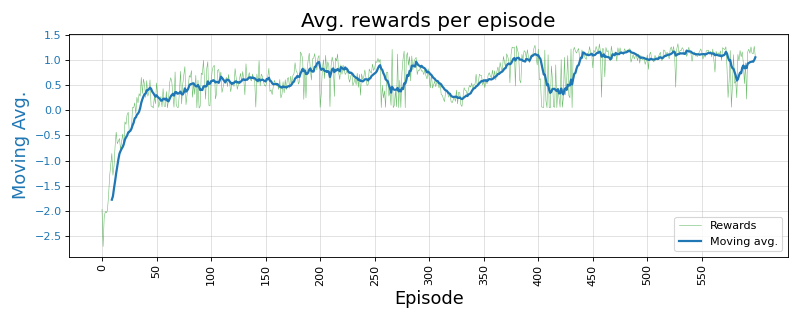
\includegraphics[width=.8\linewidth]{images\Dasic_HighNBD_Avg_episode_rewards.png}  
%		\caption{Put your sub-caption here}
%		\label{fig:sub-first}
%	\end{subfigure}
%	\begin{subfigure}{.5\textwidth}
%		\centering
%		% include second image
%		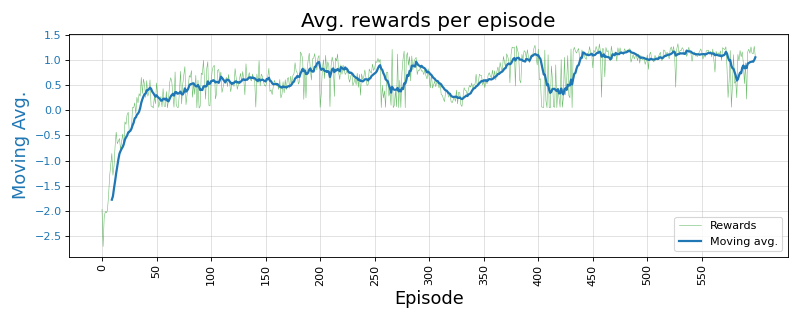
\includegraphics[width=.8\linewidth]{images\Dasic_HighNBD_Avg_episode_rewards.png}  
%		\caption{Put your sub-caption here}
%		\label{fig:sub-second}
%	\end{subfigure}
%	\caption{Put your caption here}
%	\label{fig:fig}
%\end{figure}



\section{Discussion}

\section{Conclusion}


%% References
\bibliography{ES_bibliography}
\end{document}
